\chapter{ELECTROMAGNETIC INDUCTION}
\section{Magnetic Flux}
Magnetic flux is a measurement of total magnetic field which passes through a given area. It is the product of the average magnetic field times the perpendicular area that it penetrates.Consider a uniform magnetic field passing through a surface S, as shown in Figure .\ref{magnetic flux}.\\
\begin{minipage}{0.75\textwidth}
	\begin{align}
	\intertext{Let the area vector be ${\vec{A}}=A \hat{{n}}$, where $A$ is the area of the surface and $\hat{{n}}$ its unit normal. The magnetic flux through the surface is given by,}
	\Phi_{B}&=\vec{{B}} \cdot \vec{{A}}=B A \cos \theta
	\intertext{Where $\theta$ is the angle between $\vec{{B}}$ and $\hat{{n}}$. If the field is non-uniform, $\Phi_{B}$ then becomes,}
	\Phi_{B}&=\iint_{S} \overrightarrow{{B}} \cdot d \vec{{A}}
	\intertext{The SI unit of magnetic flux is the weber $({Wb})$ :}\notag
	1 \mathrm{~Wb}&=1 \mathrm{~T} \cdot \mathrm{m}^{2}
	\end{align}
\end{minipage}
\begin{minipage}{0.25\textwidth}
	\begin{figure}[H]
		\centering
		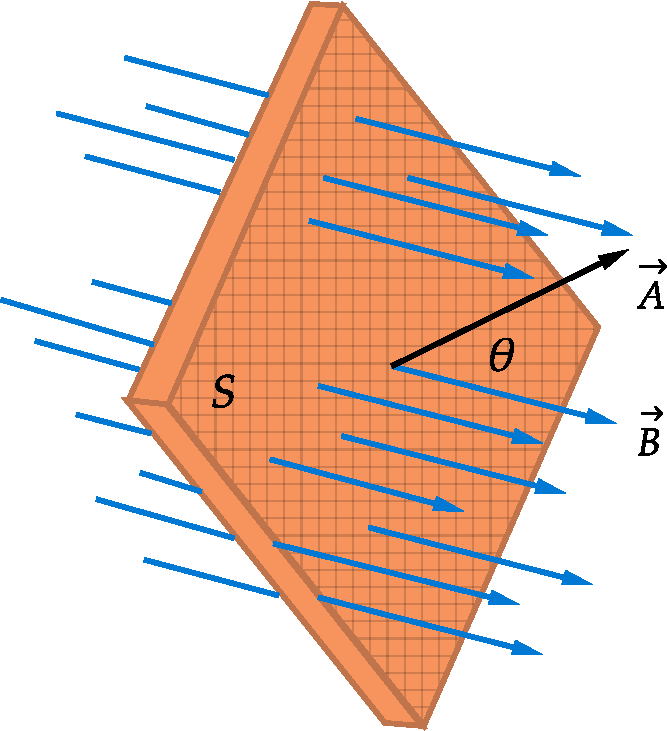
\includegraphics[height=4cm,width=5cm]{magneticflux}
		\caption{Magnetic flux.}
		\label{magnetic flux}
	\end{figure}
\end{minipage}


\section{Electromotive Force }
\section{Motional emf}
\par When we consider static electric field $E$, the potential difference between any two point $a$ and $b$ is given $$v=-\int_{a}^{b} E\cdot dl$$
\begin{flushright}
	\begin{minipage}{0.20\textwidth}				
		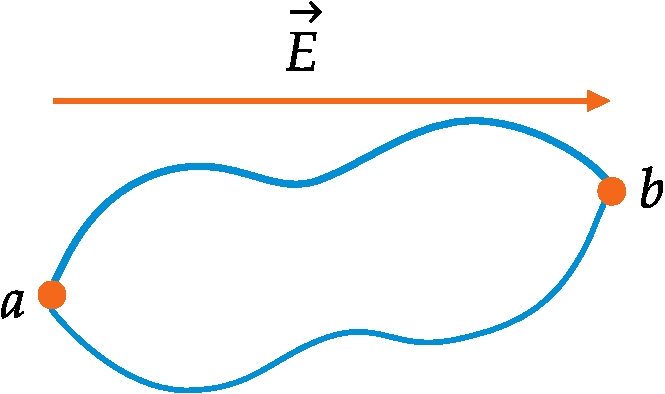
\includegraphics[width=0.85\textwidth]{diagram-20210427(3)-crop}
	\end{minipage}
\end{flushright}
And work done by the electric field along a closed path is zero.
\begin{align*}
i.e., \quad \oint E\cdot dl&=0\\
\rightarrow \quad \nabla \times E&=0
\end{align*}
\begin{minipage}{.45\textwidth}
	\begin{center}
		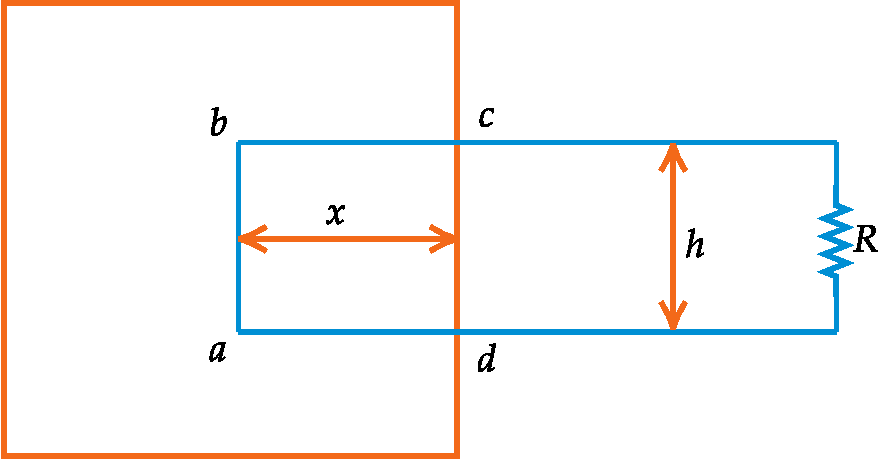
\includegraphics[width=0.7\textwidth]{diagram-20210426(1)-crop}
	\end{center}
\end{minipage}\\
\\Suppose the magnetic field $B$ in the shaded region is pointing in to the page, we are moving a wire having a resistor connected at the end through the field towards right with a speed $v$, the charges in the segment $a$\ $b$ experience a magnetic force (Lorentz force) whose vertical component $qvB$ drives a current around the loop in the clockwise direction, so the e.m.f generated,

\begin{align*}
\varepsilon&=\oint F_{mag} \cdot dl 
\intertext{Here $F_{mag}$ is the magnetic Lorentz force per unit charge. We know that,}
 {F_{Lorentz}}&=q(v\times B)
 \intertext{Since $q=1\ $\ unit and,\ $ v $ \ and $ B $\  are $ \perp^{lr} $}
F_{mag}&=vB\\
\varepsilon&=\oint F_{mag}\cdot dl\\
\varepsilon&=\oint vB\cdot dl\\
\varepsilon&= vBh \hspace{2cm}\text{$\oint  dl=h$ $ \rightarrow $ width of the loop}
\intertext{If $\phi$ is the flux of $B$ through the shaded region }
\phi=&\int B \cdot da\quad\rightarrow da=hx\\
=&Bhx
\intertext{When the  loop moves, flux decreases.}
\frac{d\phi}{dt}&=Bh\frac{dx}{dt}=-Bhv \hspace{2cm}\rightarrow\frac{dx}{dt}=-v\\
\frac{d\phi}{dt}&=-Bhv
\intertext{Thus precisely the emf generated in the loop is the negative rate of change of flux through the loop. } 
\varepsilon&=\frac{-d \phi}{dt}
\intertext{This is called \textbf{Flux rule} for motional emf.}
\end{align*}

\subsection{Fleming's Right Hand Rule}
The Fleming's right hand rule is used to determine the direction of induced current. Accorrding to this rule, stretch the thumb, forefinger and centre finger of right hand in mutually perpendicular directions such that the forefinger points in the direction of magnetic field and thumb is along the direction of motion of the conductor, the centre finger will point in the direction of the induced current.
\begin{exercise}
	A metal stock of length, $2 m/s$ moves with speed $2 m/s$ in a direction making $30^{\circ}$ with its length. If a magnetic field of $0.2$ Tesla exists in the region perpendicular to the rod then p.d developed between it's ends is........ volts.
\end{exercise}
\begin{answer}
	The potential difference developed between the ends of the rods is,\\ 
	\begin{minipage}{0.60\textwidth}\hfill
		\begin{align*}
		\varepsilon&=B l v \sin \theta\\
		&=0.2 \times 2 \times 2 \times \sin 30 \\
		&=0 .4 \text{ volt}\\
		\end{align*}
	\end{minipage}
	\begin{minipage}{0.40\textwidth}\hfill
		\begin{align*}
		\theta&=30^{\circ}\\
		l&=2 m\\
		v&=2 m/s\\
		B&=0.2 \text{ Tesla}
		\end{align*}
	\end{minipage}
\end{answer}
\subsection{Faraday's law}
The electric fields and magnetic fields considered , produced by stationary charges and moving charges (currents), respectively. Imposing an electric field on a conductor gives rise to a current which in turn generates a magnetic field.  In 1831, Michael Faraday discovered that, by varying magnetic field with time, an electric field could be generated. The phenomenon is known as electromagnetic induction.
\begin{figure}[H]
	\begin{minipage}{0.30\textwidth}
	\centering
	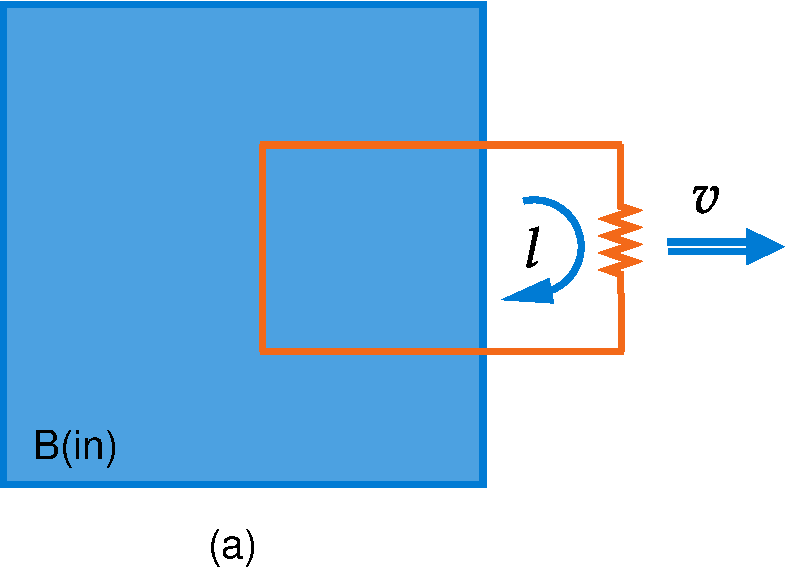
\includegraphics[height=3.2cm,width=5cm]{faraday1}
	\end{minipage}
\begin{minipage}{0.30\textwidth}
	\centering
	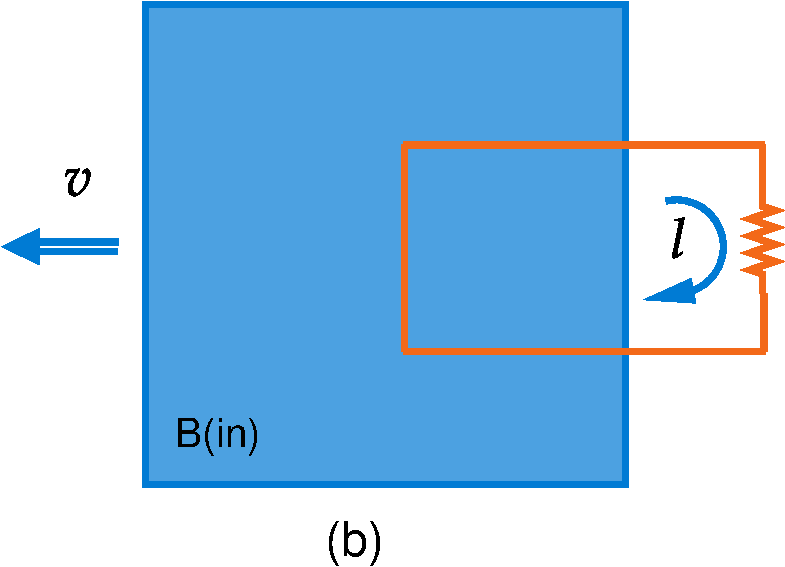
\includegraphics[height=3.2cm,width=5cm]{faraday2}
\end{minipage}
\begin{minipage}{0.30\textwidth}
	\centering
	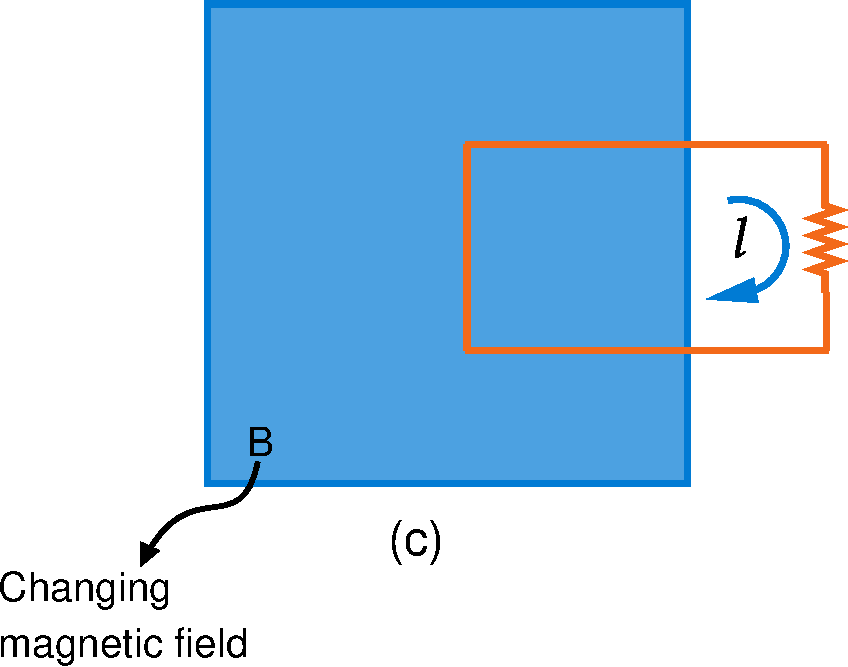
\includegraphics[height=3.7cm,width=5cm]{faraday3}
\end{minipage}
\caption{Faraday's Experiment.}
\end{figure}
Faraday's experiment demonstrates that an electric current is induced in the loop by changing the magnetic field. The coil behaves as if it were connected to an emf source. It is found that the induced emf depends on the rate of change of magnetic flux through the coil.\\
An emf is generated in loop if,\\\\
\textbf{1.}
If you pull a loop of wire through a magnetic field. 
\begin{align*}
\intertext{In the first case emf is induced due to change in flux exposed by flux rule.}
\varepsilon&=\frac{-d\phi}{dt}
\intertext{Here the emf is magnetic that is emf is induced by Lorentz force.}
\end{align*}
\textbf{2.}
If you move the magnet near a loop holding the loop still.\\\\
There will be no motion of charges since the loop is at rest so the force can't be magnetic. Here the reason for emf is the electric field which is induced by the changing magnetic field.
\begin{align*}
\varepsilon=\oint E\cdot dl&=\frac{-d\phi}{dt}\\
\oint E\cdot dl&=-\oint \frac{dB}{dt}\cdot da
\intertext{By applying Stoke's theorem}
\nabla\times E&=\frac{-dB}{dt}\\
\end{align*}
\textbf{3.}
Changing the magnetic field by keeping the loop and the magnet at rest.\\\\
Magnetic and loop are moving giving rise to an emf, $ \frac{-d\phi}{dt} $
\begin{align*}
\intertext{Now the those cases summerise in to a single form}
\varepsilon&=\frac{-d\phi}{dt}
\end{align*}

The direction of the induced current is given by Lenz's law.
\subsection{Lenz's law }
The direction of the induced current in electromagnetic induction is given by Lenz's law.\\
\begin{definition}
The induced current produces magnetic fields which tend to oppose the change in magnetic flux that induces such currents.\\
\end{definition}
\textbf{\large Explanation:}\\
\begin{minipage}{.60\textwidth}
	\begin{center}
		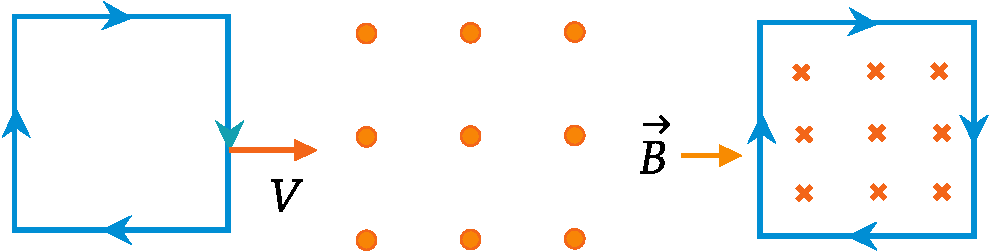
\includegraphics[height=2cm,width=9cm]{04-crop}
	\end{center}
\end{minipage}\\\\\\
Suppose we have a coil which is moving towards a constant magnetic field pointing out of the page. When it reaches the field the flux in it is increasing. So there should be an induced current in the loop. Since the flux is increasing the induced current will flow. In such a way that the magnetic field produced by it should oppose the original field. So inside the coil the field must pointing in to the page. Therefore current must flow in clockwise direction.\\\\
\begin{minipage}{.60\textwidth}
	\begin{center}
		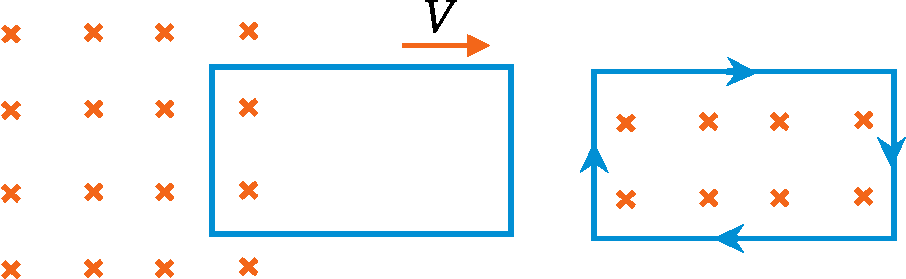
\includegraphics[height=2.5cm,width=8cm]{05-crop}
	\end{center}
\end{minipage}\\\\
Consider a loop which is initially in a magnetic field pointing into the page. Now we are moving it towards right with a velocity $V$. Now the flux in it is going to decrease. So magnetic field should be produced in such a way that it will oppose the change. So the magnetic field should be produced in the same direction as the original one. So it must be pointing into the page inside the coil. Therefore the current must flow in clockwise direction.\\\\\	Lenz's Law is not a fundamental law. It is a direct consequence that comes from both Fleming's Right and Left Hand rules . Fleming's Rules are the most fundamental principles of charge/field/motion/force interaction.
\begin{note}
The Right Hand (generator) Rule shows the direction of the induced emf and the resulting(conventional) current. This is all you need to find the direction of induced current. (Just remember that it is conventional current and it is really the emf that is induced and that a current will flow if there is a conduction path)\\
The Left Hand (motor) Rule shows the direction of the force that results from the above current and, therefore the opposition force to the original movement.\\
The latter will be seen as opposition to the original
	movement, when you apply everything correctly. This is Lenz's Law.\\\\
	To apply this:
\\	Pick a point on the conductor.\\
Given the magnetic field and motion at that point, use the Right hand Rule to determine the induced current direction.\\
At that point, given the field and current, use the Left Hand Rule to determine the resulting force. It will be opposite to the original motion.
\end{note}
\subsection{ Various formulae of induced EMF}
\begin{enumerate}
	\item  When a conducting rod of length $L$ is rotated in a perpendicur field of strength $B$, the induced emf generated is
	\begin{minipage}{0.5\textwidth}
	$$
	\begin{aligned}
	&e=-\frac{B \omega L^{2}}{2}=\frac{-B(2 \pi n) L^{2}}{2} \\
	&e=-B n\left(\pi L^{2}\right)=-B n A
	\end{aligned}
	$$
	\end{minipage}
\begin{minipage}{0.5\textwidth}
	\begin{figure}[H]
	\begin{center}
		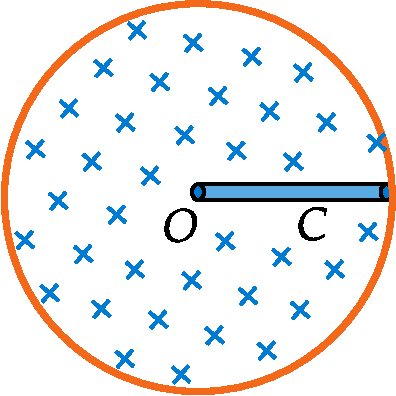
\includegraphics[width=0.25\textwidth]{emf}
	\end{center}
\end{figure}
\end{minipage}
	where $\omega$ is angular frequency and $n$ is frequency of $\operatorname{rod} A=\pi L^{2}$.
	\item When a conducting solid disc of radius $r$ is rotating with a uniform angular velocity $\omega$ in a perpendicular magnetic field $B$, the emf induced between the centre and rim of disc is
	$$
	e=\frac{-B \omega r^{2}}{2}=-B n A
	$$
	If rotation is anticlockwise, then -ve charge accumulates at the rim and +ve charge accumulates at the centre.
	\item When a conducting rod of length $l$, moves with a velocity $v$ in a uniform magnetic field $B$, the induced emf is $e=B l v \sin \theta$,
	\item When a coil moves linearly in a uniform magnetic field, but it remains wholly within the field, $d \phi=0$. $\therefore e=0 .$ However, when the coil enters the field partially or leaves the field partially, flux linked with the coil changes and induced emf $e=B l v$ develops.
\end{enumerate}
\begin{exercise}
	A conducting rod of length $l$ is rotated with uniform angular velocity $\omega$ about one end in uniform magnetic field $B$. Electric field induced inside the rod at a distance $x$ from fixed end is ?
\end{exercise}
\begin{answer}
	\opencutright
	\renewcommand\windowpagestuff{
		\centering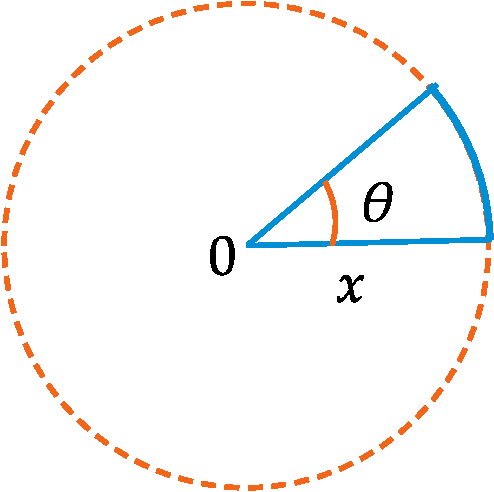
\includegraphics[width=3cm]{06-crop}}
	\begin{cutout}{3}{\dimexpr\linewidth-10cm\relax}{0pt}{2}
		\begin{align*}
		 \ \text{emf at a distance x,}\\
		\text{From center ,}\  \varepsilon&=\frac{-d \phi}{d t}\\
		&=-\frac{B \cdot d A}{d t}\\
		\text{Area} &=\frac{1}{2} x^{2} \theta \\
		\frac{d A}{d t}&=\frac{1}{2} x^{2} \frac{d \theta}{d t} \hspace{2cm}\frac{d \theta}{d t}=\omega\\
		&=\frac{1}{2} x^{2}\omega\\
		\varepsilon&=\frac{-1}{2} B x^{2}\omega\\
		\text{Electric field at $x$ , }\ E&=\frac{-d v}{d x}\\
		&=\frac{1}{2} B\omega\frac{d x^{2}}{d x}\\
		&=B\omega x
		\end{align*}
	\end{cutout}
\end{answer}
\begin{exercise}
	A uniform magnetic field $\vec{B}(t)$, pointing straight up, fills the shaded circular region. If $B$ is changing with time, what is the induced electric field?\\
	\begin{minipage}{.45\textwidth}
		\begin{center}
			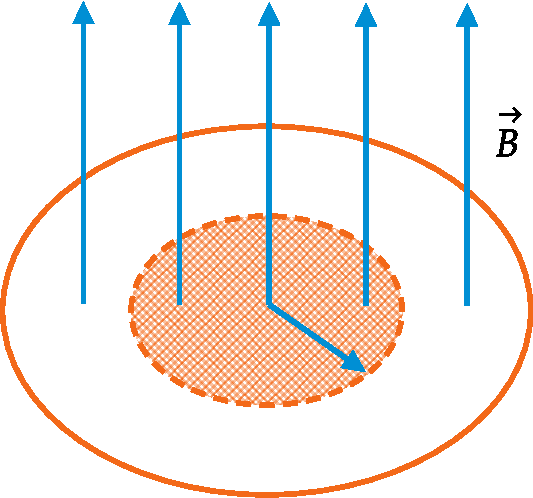
\includegraphics[width=0.4\textwidth]{diagram-20210426(2)-crop}
		\end{center}
	\end{minipage}\\
\end{exercise}
\begin{answer}
	$\vec{E}$ points in the circumferential direction, just like the magnetic field inside a long straight wire carrying a uniform current density. Draw an Amperian loop of radius $s$, and apply Faraday's law:
	\begin{align*}
	\oint \vec{E} \cdot d \vec{l}&=E(2 \pi s)\\&=-\frac{d \Phi}{d t}\\&=-\frac{d}{d t}\left(\pi s^{2} B(t)\right)\\&=-\pi s^{2} \frac{d B}{d t}
	\intertext{	Therefore}
	E(2 \pi s)&=-\pi s^{2} \frac{d B}{d t}\\
	\vec{E}&=-\frac{s}{2} \frac{d B}{d t} \hat{\boldsymbol{\phi}}
	\intertext{If $\vec{B}$ is increasing, $\vec{E}$ runs clockwise, as viewed from above.}
	\end{align*}
\end{answer}
\subsection{Mutual Inductance and Self Inductance}
\subsection{Mutual Inductance}
We have two loops $1$ and $2$ as shown in the figure.\ref{mutual inductance}. Suppose the current flowing through the loop $1$ is $I_1$, it produces a magnetic field $B_1$ which is propotional to current $I_1$ by Biot-Savart law.\\
\begin{minipage}{0.65\textwidth}
	\begin{align*}
B_1&=\frac{\mu_{0}}{4\pi}I_1\oint \frac{dl \times\hat{r}}{r^2}
\intertext{These field lines pan through second loop and flux through it is $\phi_2$}
\phi_2&=\oint B_1 \cdot da_2\\
\text{So,} \ \phi_2 &\propto  I_1\\
\phi_2&=M_{21}I_1 
\intertext{$M_{21}$ is constant of proportionality, is called as mutual inductance of the two loops,}
\phi_2&=\int B_1\cdot da_2\\
\text{But,} \ B_1&=\nabla\times A_1 \hspace{0.6cm} 
\text{$A_1$ is the magnetic vector potential.} \\
\therefore\phi_2&=\int\nabla \times A_1\cdot da_2\\
\text{By Stoke's theorem,}\ \phi_2&=\oint A_1\cdot dl_2 
\end{align*}
	
\end{minipage}
\begin{minipage}{0.20\textwidth}
\begin{figure}[H]
	\centering
	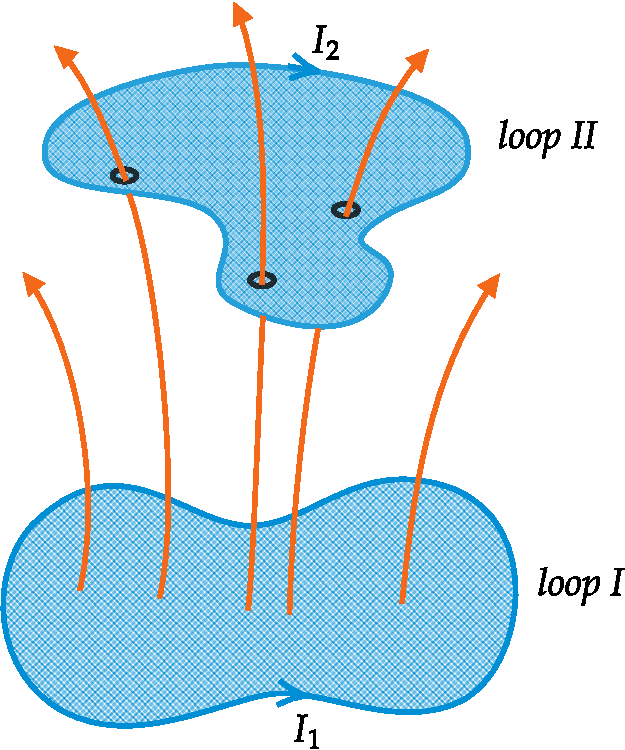
\includegraphics[height=5cm,width=5cm]{diagram-20210426(3)-crop}
	\caption{}
	\label{mutual inductance}
\end{figure}
\end{minipage}
\begin{align*}
\intertext{Magnetic vector potential due to small length element $dl$ can be calculated as,}
A_1&=\frac{\mu_{0} I_1}{4\pi}\oint \frac{dl_1}{r}\\
\therefore\phi_2&=\frac{\mu_{0}I_1}{4\pi}\oint\left( \oint\frac{dl}{r}\right) dl_2 \\
\intertext{Comparing  both equations for $\phi_2$  we  get,}\\
M_{21}&=\frac{\mu_{0}}{4 \pi}\oint \oint \frac{dl_1 \cdot dl_2}{r}\quad\Rrightarrow\quad\text{Neumann formula}
\end{align*}

\begin{note}\\
	\textbf{(a.)} 	Mutual Inductance is a geometrical quantity depends only on the size , shape and relative positions of the two loops. \\\\
	\textbf{(b.)} If we change the rules of loop $1$ and $2$ we will get the same equation as $M_{21}$\ for\ $M_{12}$.
\end{note}
\begin{align*}
M_{12}&=\frac{\mu_{0}}{4 \pi}\oint \oint \frac{dl_1 \cdot dl_2}{r}\\
M_{12}&=M_{21}\hspace{1cm} \text{Let's say  M} \\
\end{align*}
Now suppose if we vary the current $I$ in loop $1$ . An emf is induced in loop $2$ By Faraday's law,
\begin{align*}
\varepsilon_2&=\frac{-d\phi_2}{dt}\\
\phi_2&=\mu_{0}I_1\\
\varepsilon_2&= -M \frac{dI_1}{dt}
\end{align*}
Whenever we vary the current through the loop $1$ an $emf$ is induced in second loop without any actual contact between them.\\
\subsection{Self Inductance}
Suppose, instead of two circuits,we  have just a
single loop and we change current in that loop. This change in current changes the magnetic field
associated with the current and the flux changes.
The given loop itself will intercept the flux and the
changing flux would result in an emf in the circuit itself.

\begin{align*}
\phi & \propto I\\
\therefore \phi&= LI
\end{align*}
Where $L$ is called self inductance,and its value depends on the geometry of the loop only. The $emf$ generated when the current changes is given by\\
\begin{align*}
\varepsilon&=\frac{-d\phi}{dt}\\
\varepsilon&=\frac{-Ld\phi}{dt} \hspace{1cm}\text{Unit of $L$ is Henries(H)}\\
1 H&=1 V.S/Ampere
\end{align*}
By Lenz's law we can say that direction of induced $emf$ is opposite to the direction of original current .Therefore it is also called Back emf.
\subsubsection{Self inductance of a solenoid.}
Consider a solenoid has a length $l$, number of turns $N$ and area of cross section $A$. The  self inductance $L$ of the solenoid is given as,\\
\begin{minipage}{0.65\textwidth}
	\begin{align*}
	B&=\mu_{0}n I\hspace{1cm}n=\frac{N}{l}\\
	&=\frac{{\mu_{0}NI}}{l}\\
	\phi&=N B A=\frac{\mu_{0} N^{2} I A}{l}\\
	\phi&=L I\\
	\therefore L I&=\frac{\mu_{0} N^{2} I A}{l}\\
	\therefore L &=\frac{\mu_{0} N^{2}  A}{l}
	\end{align*}
\end{minipage}
\begin{minipage}{0.35\textwidth}
	\begin{figure}[H]
		\centering
		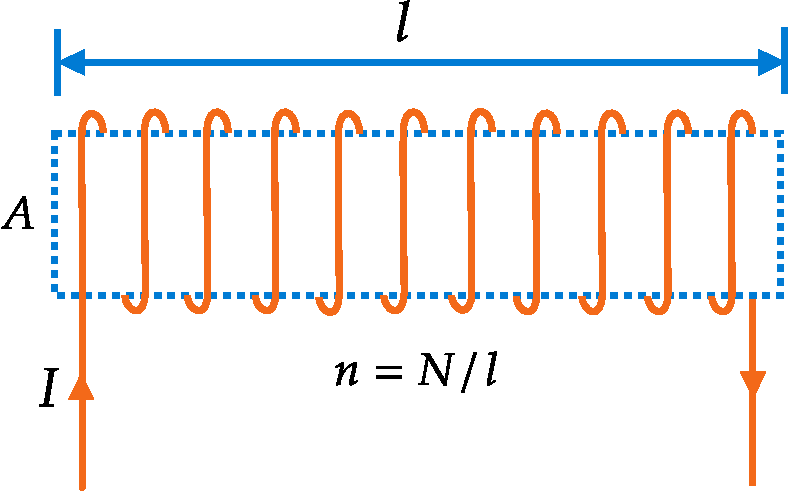
\includegraphics[height=3cm,width=5cm]{solenoid}
		\caption{Solenoid}
		\label{Solenoid}
	\end{figure}
\end{minipage}
\begin{exercise}
	A current $l$ is flowing in a toroidal coil of circular cross section of radius $R$ with $N$ number of turns distributed uniformly over its circumference if $A$ is the cross sectional area of the toroid, $I B$ Self inductance will be
\end{exercise}
\begin{answer}
	\begin{align*}
	B&=\frac{\mu_{0} N I}{2 \pi R}\\
	\phi&=N B A=\frac{\mu_{0} N^{2} I A}{2 \pi R}\\
	\phi&=L I\\
	L I&=\frac{\mu_{0} N^{2} I A}{2 \pi R}\\
	\therefore L&=\frac{\mu_{0} N^{2}  A}{2 \pi R}
	\end{align*}
\end{answer}
\subsection{Combination of inductors}
\begin{enumerate}
	\item When two coils are connected in series and current in both is in the same direction,
	$$
	L=L_{1}+L_{2}+2 M
	$$
	When current in the two coils flows in opposite directions.
	$$
	L=L_{1}+L_{2}-2 M
	$$
	If we take $M=0$, then
	$$
	L=L_{1}+L_{2}
	$$
	\item When two coils are connected in parallel, then
	$$
	\begin{aligned}
	&\frac{1}{L}=\frac{1}{\left(L_{1}+M\right)}+\frac{1}{\left(L_{2}+M\right)} \\
	&L=\frac{L_{1} L_{2}+M^{2}+M\left(L_{1}+L_{2}\right)}{L_{1}+L_{2}+2 M}
	\end{aligned}
	$$
	$M=0$\\
	$$L=\frac{L_{1} L_{2}}{L_{1}+L_{2}}$$
\end{enumerate}
\newpage
\begin{abox}
	Practice set 1
	\end{abox}
\begin{enumerate}
	\begin{minipage}{\textwidth}
		\item Consider a conducting loop of radius $a$ and total loop resistance $R$ placed in a region with a magnetic field $B$ thereby enclosing a flux $\phi_{0}$. The loop is connected to an electronic circuit as shown, the capacitor being initially uncharged\\
		\begin{figure}[H]
			\centering
			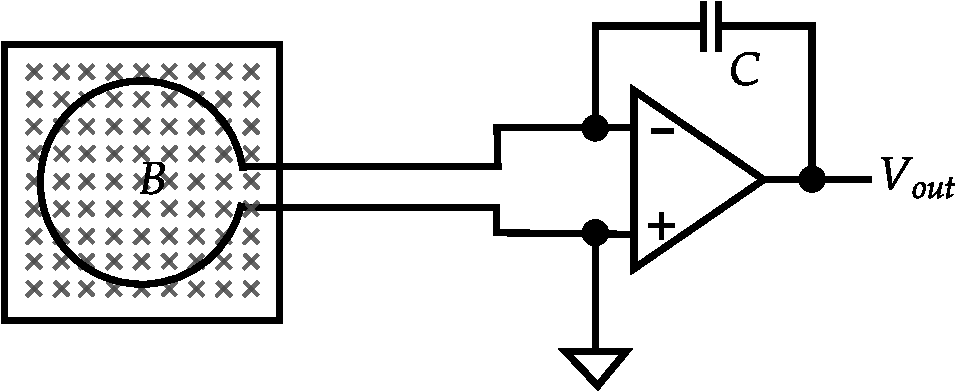
\includegraphics[height=3cm,width=5cm]{diagram-20210817(14)-crop}
		\end{figure}
		If the loop is pulled out of the region of the magnetic field at a constant speed $u$, the final output voltage $V_{\text {out }}$ is independent of
		\exyear{GATE 2010}
	\end{minipage}
	\begin{tasks}(4)
		\task[\textbf{A.}] $\phi_{0}$
		\task[\textbf{B.}]$u$ 
		\task[\textbf{C.}]$R$
		\task[\textbf{D.}] $C$ 
	\end{tasks}
\begin{minipage}{\textwidth}
	\item A circular loop made of a thin wire has radius $2 \mathrm{~cm}$ and resistance $2 \Omega$. It is placed perpendicular to a uniform magnetic field of magnitude $\left|\vec{B}_{0}\right|=0.01$ Tesla. At time $t=0$ the field starts decaying as $\vec{B}=\vec{B}_{0} e^{-t / t_{0}}$, where $t_{0}=1 s .$ The total charge that passes through a cross section of the wire during the decay is $Q$. The value of $Q$ in $\mu C$ (rounded off to two decimal places) is
	\exyear{GATE 2019}
\end{minipage}
\begin{minipage}{\textwidth}
	\item A circular conducting ring of radius $R$ rotates with constant angular velocity $\omega$ about its diameter placed along the $x$-axis. A uniform magnetic field $B$ is applied along the $y$-axis. If at time $t=0$ the ring is entirely in the $x y$-plane, the emf induced in the ring at time $t>0$ is
	\exyear{JEST 2012}
\end{minipage}
\begin{tasks}(2)
	\task[\textbf{A.}] $B \omega^{2} \pi R^{2} t$
	\task[\textbf{B.}]$B \omega \pi R^{2} \tan (\omega t)$
	\task[\textbf{C.}]$B \omega \pi R^{2} \sin (\omega t)$
	\task[\textbf{D.}]$B \omega \pi R^{2} \cos (\omega t)$
\end{tasks}
\begin{minipage}{\textwidth}
	\item Two parallel rails of a railroad track are insulated from each other and from the ground. The distance between the rails is 1 meter. A voltmeter is electrically connected between the rails. Assume the vertical component of the earth's magnetic field to the $0.2$ gauss. What is the voltage developed between the rails when a train travels at a speed of $180 \mathrm{~km} / \mathrm{h}$ along the track? Give the answer in milli-volts.
	\exyear{JEST 2018}
\end{minipage}
\begin{minipage}{\textwidth}
	\item A circular metal loop of radius $a=1 \mathrm{~m}$ spins with a constant angular velocity $\omega=20 \pi \mathrm{rad} / \mathrm{s}$ in a magnetic field $B=3$ Tesla, as shown in the figure. The resistance of the loop is 10 ohms. Let $P$ be the power dissipated in one complete cycle.
\begin{figure}[H]
	\centering
	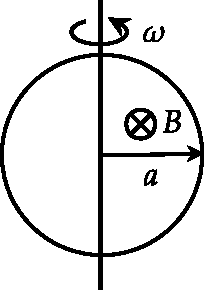
\includegraphics[height=5cm,width=5cm]{nimi2-crop}
\end{figure}
	 What is the value of $\frac{P}{\pi^{4}}$ in Watts?
	\exyear{JEST 2019}
\end{minipage}
\end{enumerate}
\colorlet{ocre1}{ocre!70!}
\colorlet{ocrel}{ocre!30!}
\setlength\arrayrulewidth{1pt}
\begin{table}[H]
	\centering
	\arrayrulecolor{ocre}
	
	\begin{tabular}{|p{1.5cm}|p{1.5cm}||p{1.5cm}|p{1.5cm}|}
		\hline
		\multicolumn{4}{|c|}{\textbf{Answer key}}\\\hline\hline
		\rowcolor{ocrel}Q.No.&Answer&Q.No.&Answer\\\hline
		1&\textbf{a}&2&\textbf{6.28}\\\hline
		3&\textbf{d}&4&\textbf{1}\\\hline
		5&\textbf{18}&&\\\hline
	\end{tabular}
\end{table}















\newpage
\begin{abox}
	Practice set 2
	\end{abox}
\begin{enumerate}
\begin{minipage}{\textwidth}
	\item A uniform magnetic field in the positive $z$-direction passes through a circular wire loop of radius $1 \mathrm{~cm}$ and resistance $1 \Omega$ lying in the $x y$-plane. The field strength is reduced from 10 tesla to 9 tesla in $1 s$. The charge transferred across any point in the wire is approximately
	\exyear{NET JUNE 2015}
\end{minipage}
\begin{tasks}(2)
	\task[\textbf{A.}]$3.1 \times 10^{-4}$ coulomb
	\task[\textbf{B.}] $3.4 \times 10^{-4}$ coulomb
	\task[\textbf{C.}] $4.2 \times 10^{-4}$ coulomb
	\task[\textbf{D.}]$5.2 \times 10^{-4}$ coulomb
\end{tasks}
\begin{minipage}{\textwidth}
	\item A magnetic field $B$ is $B \hat{z}$ in the region $x>0$ and zero elsewhere. A rectangular loop, in the $x y$-plane, of sides $l$ (along the $x$-direction) and $h$ (along the $y$ - direction) is inserted into the $x>0$ region from the $x<0$ region at constant velocity $v=v \hat{x}$. Which of the following values of $l$ and $h$ will generate the largest EMF?
	\exyear{NET JUNE 2016}
\end{minipage}
\begin{tasks}(2)
	\task[\textbf{A.}] $l=8, h=3$
	\task[\textbf{B.}]$l=4, h=6$
	\task[\textbf{C.}]$l=6, h=4$
	\task[\textbf{D.}]$l=12, h=2$
\end{tasks}
\end{enumerate}

\colorlet{ocre1}{ocre!70!}
\colorlet{ocrel}{ocre!30!}
\setlength\arrayrulewidth{1pt}
\begin{table}[H]
	\centering
	\arrayrulecolor{ocre}
	
	\begin{tabular}{|p{1.5cm}|p{1.5cm}||p{1.5cm}|p{1.5cm}|}
		\hline
		\multicolumn{4}{|c|}{\textbf{Answer key}}\\\hline\hline
		\rowcolor{ocrel}Q.No.&Answer&Q.No.&Answer\\\hline
		1&\textbf{a}&2&\textbf{b}\\\hline
	\end{tabular}
\end{table}



































